\documentclass{article}
\usepackage[italian]{babel}
\usepackage[utf8]{inputenc}
\usepackage[T1]{fontenc}
\usepackage{graphicx}
\usepackage[colorinlistoftodos]{todonotes}
\usepackage[colorlinks=true, allcolors=tudelftblue]{hyperref} %sets hyperlink colour
\usepackage{caption}
\usepackage{subcaption}
\usepackage{xcolor}
\usepackage{roboto} % for Roboto Slab font
\usepackage{float}
\usepackage{titling} 
\usepackage{blindtext}\usepackage{titlesec}
\usepackage[square,sort,comma,numbers]{natbib}
\usepackage[colorinlistoftodos]{todonotes}
\usepackage{tikz}
\usepackage{geometry}
\usepackage{sectsty}
\usepackage{amsmath}
\usepackage{tikzpagenodes}
\usepackage{booktabs}
\usepackage{listings}
\usepackage{svg}

\usepackage[labelfont=bf, labelsep=colon]{caption}
\captionsetup[table]{name=Tabella, position=bottom}
\captionsetup[figure]{name=Schema, position=bottom}


\definecolor{tudelftdarkblue}{RGB}{0,0,0}
\definecolor{tudelftcyan}{RGB}{209,65,36}
\definecolor{tudelftblue}{RGB}{99, 102, 106}
\geometry{a4paper, margin=2cm}
\allsectionsfont{\color{black}} %sets colour for all headers
\usepackage{helvet}
\renewcommand{\familydefault}{\sfdefault}
\sectionfont{\fontfamily{RobotoSlab-TLF}\selectfont}
%%%%%%%%%%%%%%%%%%%%%%%%%%%%%%%%%%%%%%%%%%%%%%%%%%%%%%%%%
\begin{document}

\begin{titlepage}
    \fontfamily{RobotoSlab-TLF}\selectfont 
%%%%%%%%%%%%%%%%%%%%%%%%%%%%%%%%%%%%%%%%%%%%%%%%%%%%%%%%%%UNCOMMENT THE FOLLOWING FOR LESS "PLAIN" TITLE PAGE (SELECT WITH MOUSE AND PRESS CTRL AND /)

    % \begin{tikzpicture}[remember picture,overlay]
    %     % Set seed for random number generator
    %     \pgfmathsetseed{4}
    %     % Define the text area to avoid
    %     \path (current page text area.south west) rectangle (current page text area.north east);
    %     % Adding circles spread over the entire page
    %     \foreach \x in {1,...,1000}
    %         \draw[tudelftdarkblue] (current page.south west) ++(rand*\paperwidth,rand*\paperheight) circle (rand*0.3);
    %     % Define coordinates for the corners of the white box
    %     \coordinate (A) at ([shift={(-8cm,12cm)}]current page.center);
    %     \coordinate (B) at ([shift={(8cm,-5cm)}]current page.center);
    %     % Draw the white background box
    %     \fill[white] (A) rectangle (B);
    %     % Adding equations as background features
    %     \node[anchor=center,rotate=20,text=tudelftcyan] at ([shift={(-7cm,-2cm)}]current page.center) {\fontsize{18}{22}\selectfont
    %     $\nabla^2 T - \frac{1}{\alpha}\frac{\partial T}{\partial t} = 0$};
    %     \node[anchor=center,rotate=-15,text=tudelftcyan] at ([shift={(5cm,-4cm)}]current page.center) {\fontsize{18}{22}\selectfont
    %     $\frac{\partial \rho}{\partial t} + \nabla \cdot (\rho \mathbf{v}) = 0$};
    %     \node[anchor=center,rotate=20,text=tudelftcyan] at ([shift={(6cm,4cm)}]current page.center) {\fontsize{18}{22}\selectfont
    %     $a^2 + b^2 = c^2$};
    %     \node[anchor=center,rotate=10,text=tudelftcyan] at ([shift={(7cm,-2cm)}]current page.center) {\fontsize{18}{22}\selectfont
    %     $E = \frac{\sigma}{\varepsilon}$};
    %     \node[anchor=center,rotate=-10,text=tudelftcyan] at ([shift={(-6cm,4cm)}]current page.center) {\fontsize{18}{22}\selectfont
    %     $F = ma$};
    %     \node[anchor=center,rotate=5,text=tudelftcyan] at ([shift={(-4cm,-5cm)}]current page.center) {\fontsize{18}{22}\selectfont
    %     $Q = -\frac{kA}{\mu} \frac{\Delta P}{L}$};
    % \end{tikzpicture}
    
%%%%%%%%%%%%%%%%%%%%%%%%%%%%%%%%%%%%%%%%%%%%%%%%%%%%%%%%%%
    \vspace*{3cm}
    
    \centering
    {\Huge \textbf{\textcolor{black}{Progetto Basi di dati}}}\\[1.5cm]
    \textsc{\LARGE Corso di Informatica}\\[0.5cm]
    \text{\large MN1-525}\\[2cm]
    
    {\Large \textbf{\textcolor{tudelftdarkblue}{Autori:}}}\\[0.5cm]
    \begin{tabular}{c}
        \Large \textcolor{tudelftdarkblue}{Bilotti Alessandro (206409)}
        % \Large \textcolor{tudelftdarkblue}{Author 2 (1234567)} \\
        % \Large \textcolor{tudelftdarkblue}{Author 3 (9876543)} \\
    \end{tabular}\\[2cm]
    
    {\Large \textcolor{tudelftdarkblue}{\today}}
    
    \vfill
    \begin{center}
        
\includegraphics[width=0.6\textwidth]{images/Logo_C_Positivo_Colore.png}
    \end{center}
\end{titlepage}

%%% Create a table of contents
\tableofcontents
\newpage

\addcontentsline{toc}{section}{Introduzione}
\section*{Introduzione}
\textbf{Greenrail\cite{Greenrail}} è un'azienda italiana, riconosciuta a livello internazionale come attore innovativo del settore ferroviario e come esempio di sviluppo industriale sostenibile secondo i principi dell'economia circolare.

\noindent Greenrail realizza i propri prodotti con plastica e gomma riciclate. Le soluzioni proposte riducono vibrazioni e impatto ambientale, aumentano la durata delle infrastrutture e possono integrare tecnologie smart (es.\ sensori o pannelli solari).

\section{Definizione dei requisiti}

\subsection{Vista Cliente}
I clienti della base dati di Greenrail rappresentano la parte finale della catena di valore, comprendono aziende e enti del settore delle infrastrutture ferroviarie. Questi possono essere gestori pubblici o privati di linee ferroviarie, imprese edili operanti su appalto pubblico, o società di progettazione infrastrutturale. I clienti devono fornire i seguenti dati: ragione sociale, tipologia (gestore, appaltatore, progettista, etc.), indirizzo (Paese, città, via, CAP), recapiti (telefono, email), codice fiscale e/o partita IVA.\\

\noindent Dopo aver consultato il catalogo dei prodotti, i clienti hanno la possibillità di effettuare richieste d’ordine, scaricare schede tecniche delle traversine, specificare i requisiti di installazione (es.\ condizioni climatiche, peso supportato, durata stimata). Per ogni ordine viene creata una commessa contenente informazioni dettagliate sul tipo di traversina scelta (Standard, Solar, LinkBox), quantità, località di destinazione ed eventuali note operative.

\noindent Il sistema tiene traccia dell'intera relazione cliente-azienda: dalle richieste iniziali di preventivo alle commesse in lavorazione, fino alla fase post-installazione. Ogni cliente ha accesso allo storico ordini e può essere associato a uno o più tecnici o partner logistici.

\subsection{Vista Produttore}
Il Produttore rappresenta il personale tecnico addetto alla realizzazione fisica delle traversine nei centri di produzione. Ogni Produttore ha un identificativo univoco, nome, cognome, qualifica, turno di lavoro, impianto di assegnazione e salario.

\noindent Il sistema consente la tracciabilità delle attività di produzione: per ogni traversina, si registrano le specifiche (variano in base al modello), la data di produzione, i materiali utilizzati, il tecnico assegnato e il numero di serie delle traversine.

\noindent I produttori devono poter visualizzare le specifiche tecniche richieste per ogni commessa, inclusi eventuali vincoli o personalizzazioni richieste dal cliente.

\noindent È inoltre previsto un registro delle non conformità rilevate in fase di produzione.

\subsection{Vista Installatore}
L’Installatore è il tecnico incaricato della posa in opera delle traversine lungo le tratte ferroviarie. Può coincidere con il Produttore o essere una figura distinta. Ogni Installatore ha un codice identificativo, nome, cognome, zona geografica di competenza, e calendario di interventi.\\

\noindent Per ogni attività di installazione, il sistema deve registrare: numedi di serie delle traversine, località di installazione, data e durrata dell'installazione. Le installazioni sono sempre collegate a una specifica commessa cliente e devono rispettare i requisiti previsti.

\noindent Il sistema deve permettere il monitoraggio degli interventi conclusi e programmati, e registrare note tecniche utili per valutazioni future.

\subsection{Vista Amministratore}
L’Amministratore è una figura di gestione centrale, responsabile del coordinamento delle operazioni e delle relazioni tra clienti, produttori e installatori.\\

\noindent L'Amministratore gestisce tutte le entità presenti: clienti, ordini, commesse, produzione e installazione.

\noindent L’Amministratore può scrivere report su quantità prodotte/installate, sostenibilità dei materiali e conformità dei certificati.

\noindent Inoltre, può intervenire per modificare dati errati, chiudere commesse, o aggiornare il catalogo prodotti.

\section{Analisi e schema scheletro}
\subsection{Analisi requisiti e schema scheletro per il Cliente}

\begin{table}[H]
    \begin{tabular}{|l|l|l|l|}
    \hline
    \textbf{Termine} & Descrizione                                                                                                      & Sinonimi                                                & Collagamenti                                                                                                  \\ \hline
    Cliente          & \begin{tabular}[c]{@{}l@{}}Enti o aziende, pubblici o privati,\\ nel settore ferroviario\end{tabular}            & \begin{tabular}[c]{@{}l@{}}Azienda,\\ Ente\end{tabular} & Prodotto, Amministratore                                                                                      \\ \hline
    Amministratore   & Coordinatore generale                                                                                            & Manager                                                 & Cliente, Prodotto                                                                                             \\ \hline
    Prodotto         & Articolo venduto da Greenrail                                                                                    & Traversina                                              & \begin{tabular}[c]{@{}l@{}}Cliente, Amministratore,\\ Produttore, Installatore,\\ Certificazione\end{tabular} \\ \hline
    Produttore       & Soggetta che realizza il prodotto                                                                                & -                                                       & Prodotto                                                                                                      \\ \hline
    Installatore     & Soggetto che installa il prodotto                                                                                & -                                                       & Prodotto                                                                                                      \\ \hline
    Certificato      & \begin{tabular}[c]{@{}l@{}}Certificazione che attesta la\\ sostenibilità e sicurezza del\\ prodotto\end{tabular} & -                                                       & Prodotto                                                                                                      \\ \hline
    \end{tabular}
    \caption{Glossario dei concetti del Cliente}
\end{table}

\begin{figure}[H]
    \centering
    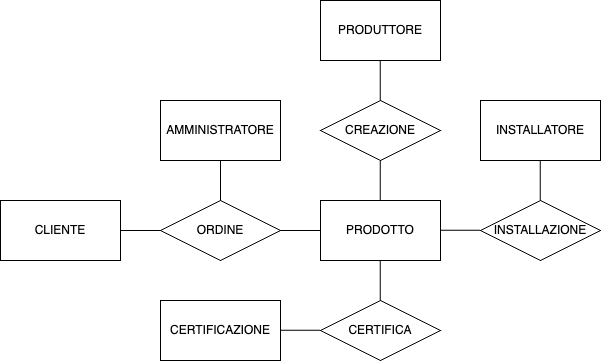
\includegraphics[width=12cm]{images/cliente.drawio.png}\\
    \caption{Schema scheletro della vista del Cliente}
\end{figure}

\subsection{Analisi requisiti e schema scheletro per il Produttore}

\begin{table}[H]
    \begin{tabular}{|l|l|l|l|}
    \hline
    \textbf{Termine} & Descrizione                                                                     & Sinonimi   & Collegamenti         \\ \hline
    Produttore       & Soggetto che realizza il prodotto                                               & -          & Sede                 \\ \hline
    Sede             & Luogo fisico                                                                    & Azienda    & Produttore           \\ \hline
    Team             & Insieme di produttori                                                           & Squadra    & Produttore, Prodotto \\ \hline
    Prodotto         & Articolo venduto da Greenrail                                                   & Traversina & Materiale, Team      \\ \hline
    Materiale        & \begin{tabular}[c]{@{}l@{}}Materiale di cui si compone un\\ prodotto\end{tabular} & -          & Fornitore, Prodotto  \\ \hline
    Fornitore        & Soggetto che fornisce materiale                                                 & -          & Materiale            \\ \hline
    \end{tabular}
    \caption{Glossario dei concetti del Produttore}
    \end{table}

\begin{figure}[H]
    \centering
    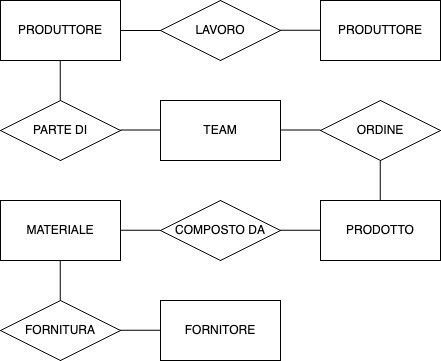
\includegraphics[width=10cm]{images/produttore.drawio.png}\\
    \caption{Schema scheletro della vista del Produttore}
\end{figure}

\subsection{Analisi requisiti e schema scheletro per l'Installatore}

\begin{table}[H]
    \begin{tabular}{|l|l|l|l|}
    \hline
    \textbf{Termine} & Descrizione                                                                                             & Sinonimi                                                 & Collegamenti                                                                 \\ \hline
    Installatore     & Soggetto che installa il prodotto                                                                       & -                                                        & Tratta, Prodotto                                                             \\ \hline
    Tratta           & Luogo dell'installazione                                                                                & Luogo                                                    & Produttore                                                                   \\ \hline
    Prodotto         & Articolo venduto da Greenrail                                                                           & Traversina                                               & \begin{tabular}[c]{@{}l@{}}Installatore, Produttore, \\ Cliente\end{tabular} \\ \hline
    Produttore       & Soggetto che realizza il prodotto                                                                       & -                                                        & Prodotto                                                                     \\ \hline
    Cliente          & \begin{tabular}[c]{@{}l@{}}Enti o aziende, pubblici o privati, \\  nel settore ferroviario\end{tabular} & \begin{tabular}[c]{@{}l@{}}Azienda, \\ Ente\end{tabular} & Prodotto                                                                     \\ \hline
    \end{tabular}
    \caption{Glossario dei concetti dell'Installatore}
\end{table}

\begin{figure}[H]
    \centering
    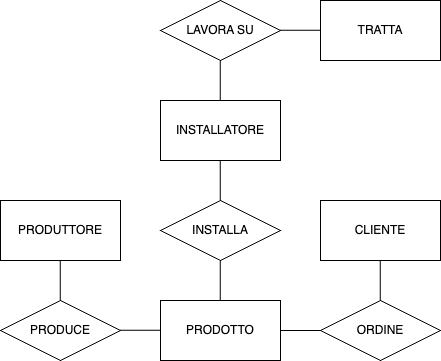
\includegraphics[width=10cm]{images/installatore.drawio.png}\\
    \caption{Schema scheletro della vista dell'Installatore}
\end{figure}

\subsection{Analisi requisiti e schema scheletro per l'Amministratore}

\begin{table}[H]
    \begin{tabular}{|l|l|l|l|}
    \hline
    \textbf{Termine} & Descrizione                                                                                             & Sinonimi          & Collegamenti                                                                                \\ \hline
    Amministratore   & Coordinatore generale                                                                                   & Manager           & \begin{tabular}[c]{@{}l@{}}Report, Sede, Team, \\ Cliente\end{tabular}                      \\ \hline
    Report           & Articolo riguardante Greenrail                                                                          & Notizia, Articolo & Amministratore                                                                              \\ \hline
    Sede             & \begin{tabular}[c]{@{}l@{}}Struttura in cui vengono costruiti\\ i prodotti Greenrail\end{tabular}       & Azienda           & Amministratore                                                                              \\ \hline
    Team             & Gruppo di persone                                                                                       & Squadra           & \begin{tabular}[c]{@{}l@{}}Amministratore, Produttori,\\ Installatori, Clienti\end{tabular} \\ \hline
    Cliente          & \begin{tabular}[c]{@{}l@{}}Enti o aziende, pubblici o privati, \\  nel settore ferroviario\end{tabular} & \begin{tabular}[c]{@{}l@{}}Azienda, \\ Ente\end{tabular} & Prodotto                                                                     \\ \hline
    Produttore       & Soggetto che realizza il prodotto                                                                       & -                 & Team, Installatori, Prodotto                                                                \\ \hline
    Installatore     & Soggetto che installa il prodotto                                                                       & -                 & Cliente, Prodotto, Team, Produttori                                                         \\ \hline
    Prodotto         & Articolo venduto da Greenrail                                                                           & Traversina        & \begin{tabular}[c]{@{}l@{}}Cliente, Installatore, Produttore,\\ Material\end{tabular}       \\ \hline
    Materiale        & \begin{tabular}[c]{@{}l@{}}Materiale di cui si compone un\\ prodotto\end{tabular}                       & -                 & Prodotto, Fornitore                                                                         \\ \hline
    Fornitore        & Soggetto che fornisce materiale                                                                         & Azienda           & Materiale                                                                                   \\ \hline
    \end{tabular}
    \caption{Glossario dei concetti dell'Amministratore}
\end{table}

\begin{figure}[H]
    \centering
    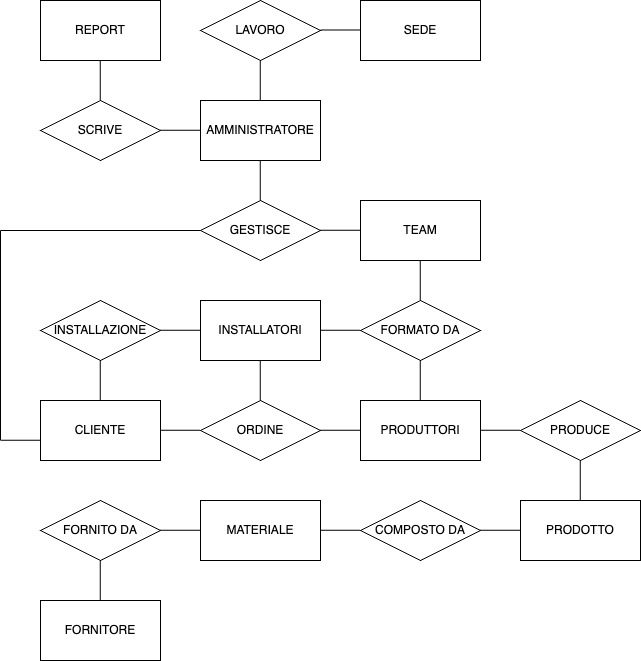
\includegraphics[width=13cm]{images/amministratore.drawio.png}\\
    \caption{Schema scheletro della vista dell'Amministratore}
\end{figure}

\section{Progettazione ed integrazione delle viste}
\subsection{Schemi E-R finali}
\subsubsection{Schema E-R del Cliente}

Nel passaggio dallo scheletro allo schema E-R finale, sono state apportate le modifiche:
\begin{enumerate}
    \item La relazione di Ordine diventa una entità, in quanto contiene informazioni aggiuntive rispetto a quelle del prodotto.
    \item L'entità Ordine viene storicizzata in Presente e Passato.
    \item Aggiunta l'istanza Modello da Prodotto per gestire i diversi modelli di traversina.
    \item L'entità Cliente generalizza i clienti Privato e Pubblico.
    \item Aggiunta l'entità Sede, generalizzazione di Sede Amministrativa e di Produzione in relazione con l'Amministratore.
\end{enumerate}

\begin{figure}[H]
    \centering
    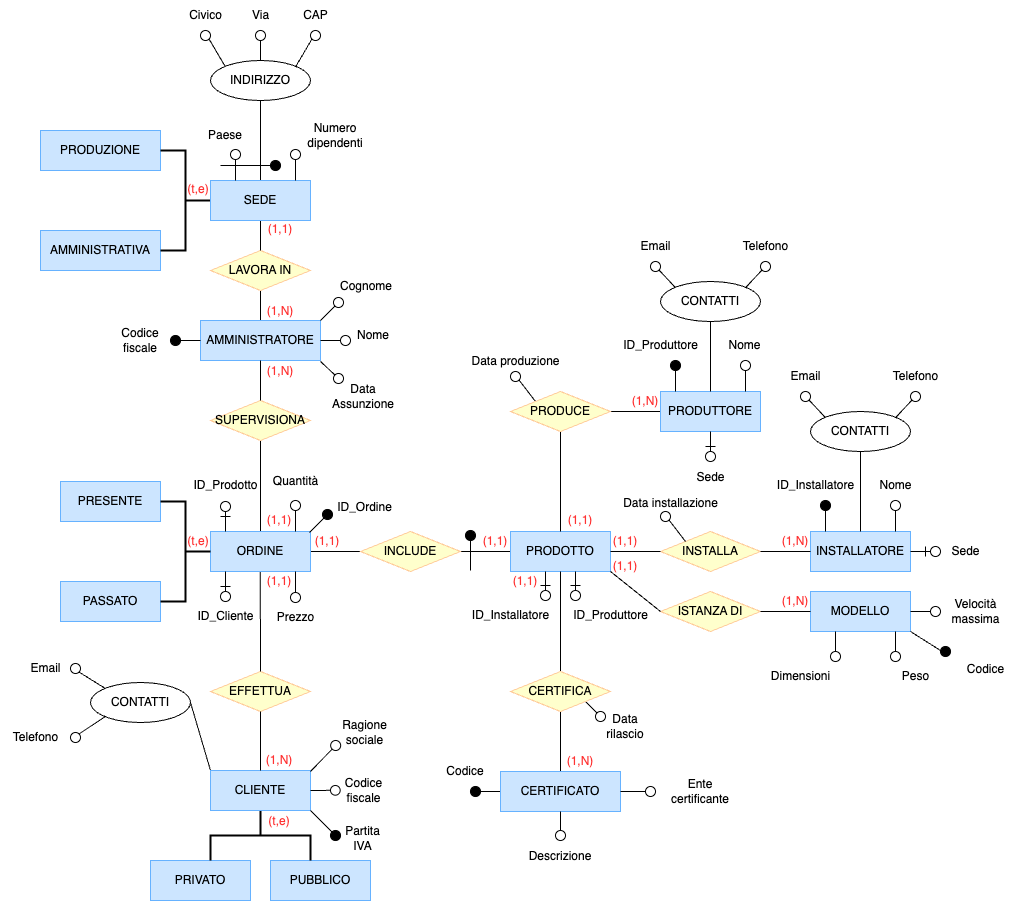
\includegraphics[width=15cm]{images/rivisto_utente.drawio.png}\\
    \caption{Schema E-R della vista del Cliente}
\end{figure}

\subsubsection{Schema E-R del Produttore}
Nel passaggio dallo scheletro allo schema E-R finale, sono state apportate le modifiche:
\begin{enumerate}
    \item Modifica dell'errata entità Produttore in Sede che generalizza i tipi di Sede Amministrativa e di Produzione.
    \item Aggiunta entità Programma contente le informazioni relative alle attività del Produttore.
    \item La relazione di Ordine diventa una entità, in quanto contiene informazioni aggiuntive rispetto a quelle del prodotto.
    \item L'entità Ordine viene storicizzata in Presente e Passato.
    \item Aggiunta l'istanza Modello da Prodotto per gestire i diversi modelli di traversina.
    \item Aggiunta l'entità 'Componente', parte di un Modello, che generalizza un 'Componente' Generico e Specifico.
\end{enumerate}

\begin{figure}[H]
    \centering
    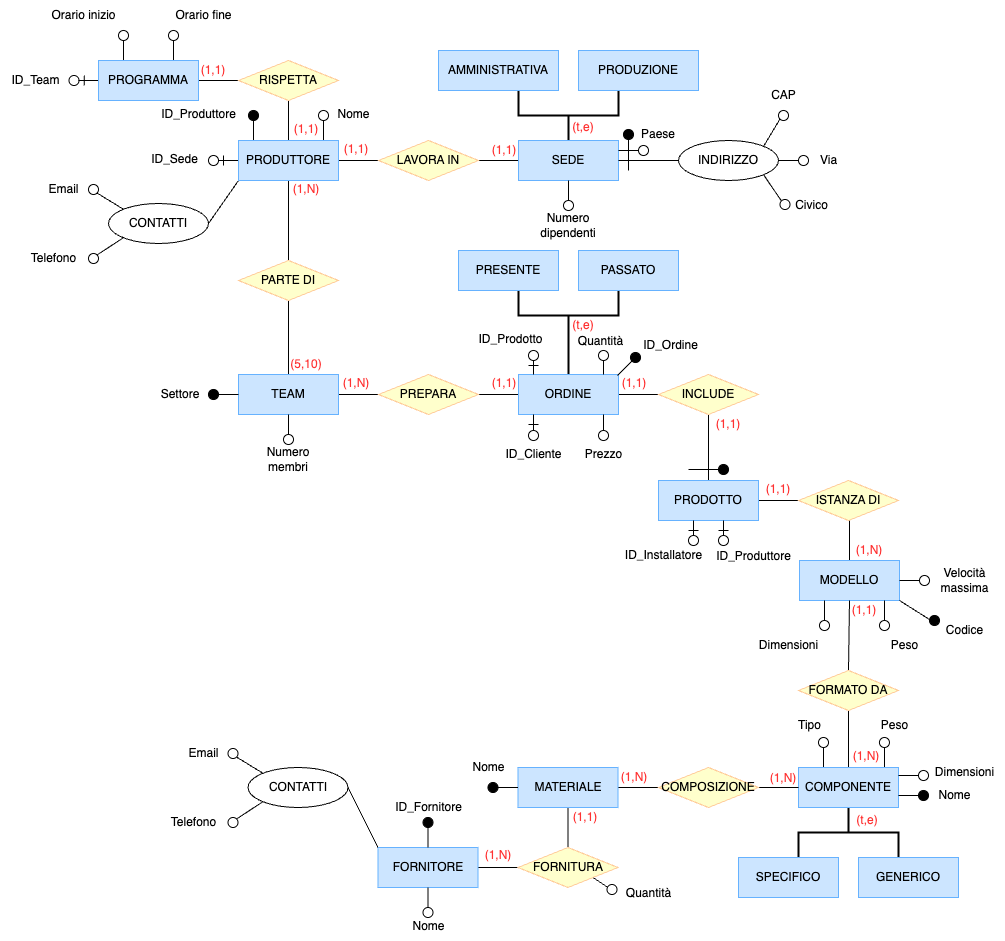
\includegraphics[width=15cm]{images/rivisto_produttore.drawio.png}\\
    \caption{Schema E-R della vista del Produttore}
\end{figure}

\subsubsection{Schema E-R dell'Installatore}
Nel passaggio dallo scheletro allo schema E-R finale, sono state apportate le modifiche:
\begin{enumerate}
    \item L'entità Tratta generalizza i tipi di Tratta Passeggeri e Merci.
    \item Come per la vista del Produttore, l'Installatore è parte di un Team.
    \item Aggiunta entità Programma contente le informazioni relative alle attività dell'Installatore.
    \item Aggiunta l'istanza Modello da Prodotto per gestire i diversi modelli di traversina.
    \item L'entità Ordine viene storicizzata in Presente e Passato.
    \item L'entità cliente generalizza i clienti Privato e Pubblico.
\end{enumerate}

\begin{figure}[H]
    \centering
    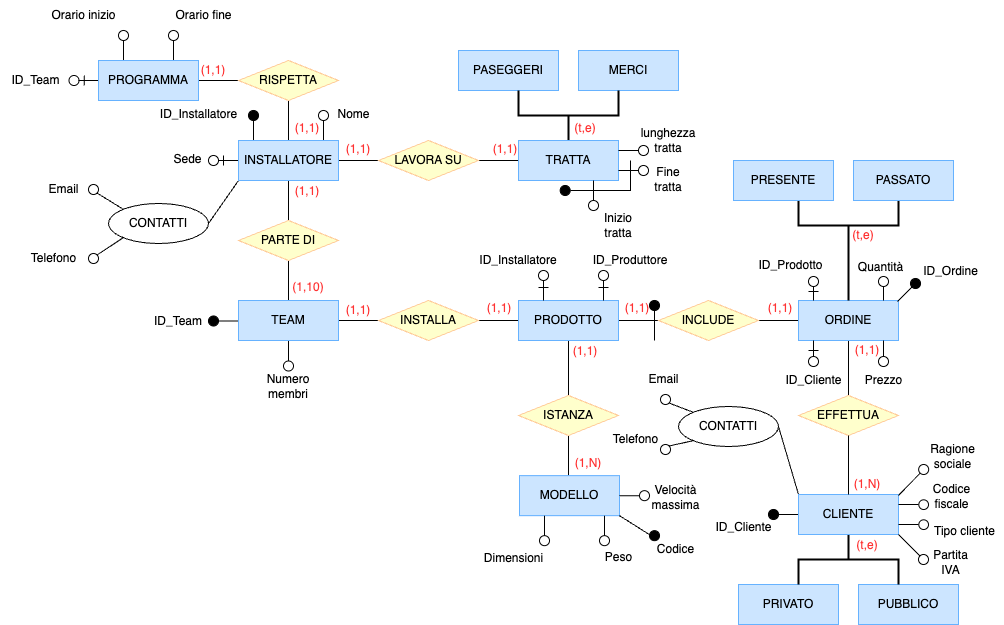
\includegraphics[width=15cm]{images/rivisto_installatore.drawio.png}\\
    \caption{Schema E-R della vista del Installatore}
\end{figure}

\subsubsection{Schema E-R dell'Amministratore}
Nel passaggio dallo scheletro allo schema E-R finale, sono state apportate le modifiche:
\begin{enumerate}
    \item L'entità Sede generalizza i tipi di Sede Amministrativa e di Produzione.
    \item Aggiunta entità Dipendente che generalizza i tipi Amministratore e Operaio.
    \item L'entità Operaio generalizza a sua volta i tipi Produttore e Installatore.
    \item L'Amministratore gestisce Team e Ordine, non più Cliente.
    \item Aggiunta l'entità Tratta che generalizza i tipi di Tratta Passeggeri e Merci.
    \item L'entità Ordine viene storicizzata in Presente e Passato.
    \item L'entità Cliente generalizza i clienti Privato e Pubblico.
    \item Aggiunta entità Certificato che certifica la sostenibilità e sicurezza del prodotto.
    \item Aggiunta l'istanza Modello da Prodotto per gestire i diversi modelli di traversina.
    \item Aggiunta entità 'Componente', parte di un Modello, che generalizza un Componente Generico e Specifico.
\end{enumerate}

\begin{figure}[H]
    \centering
    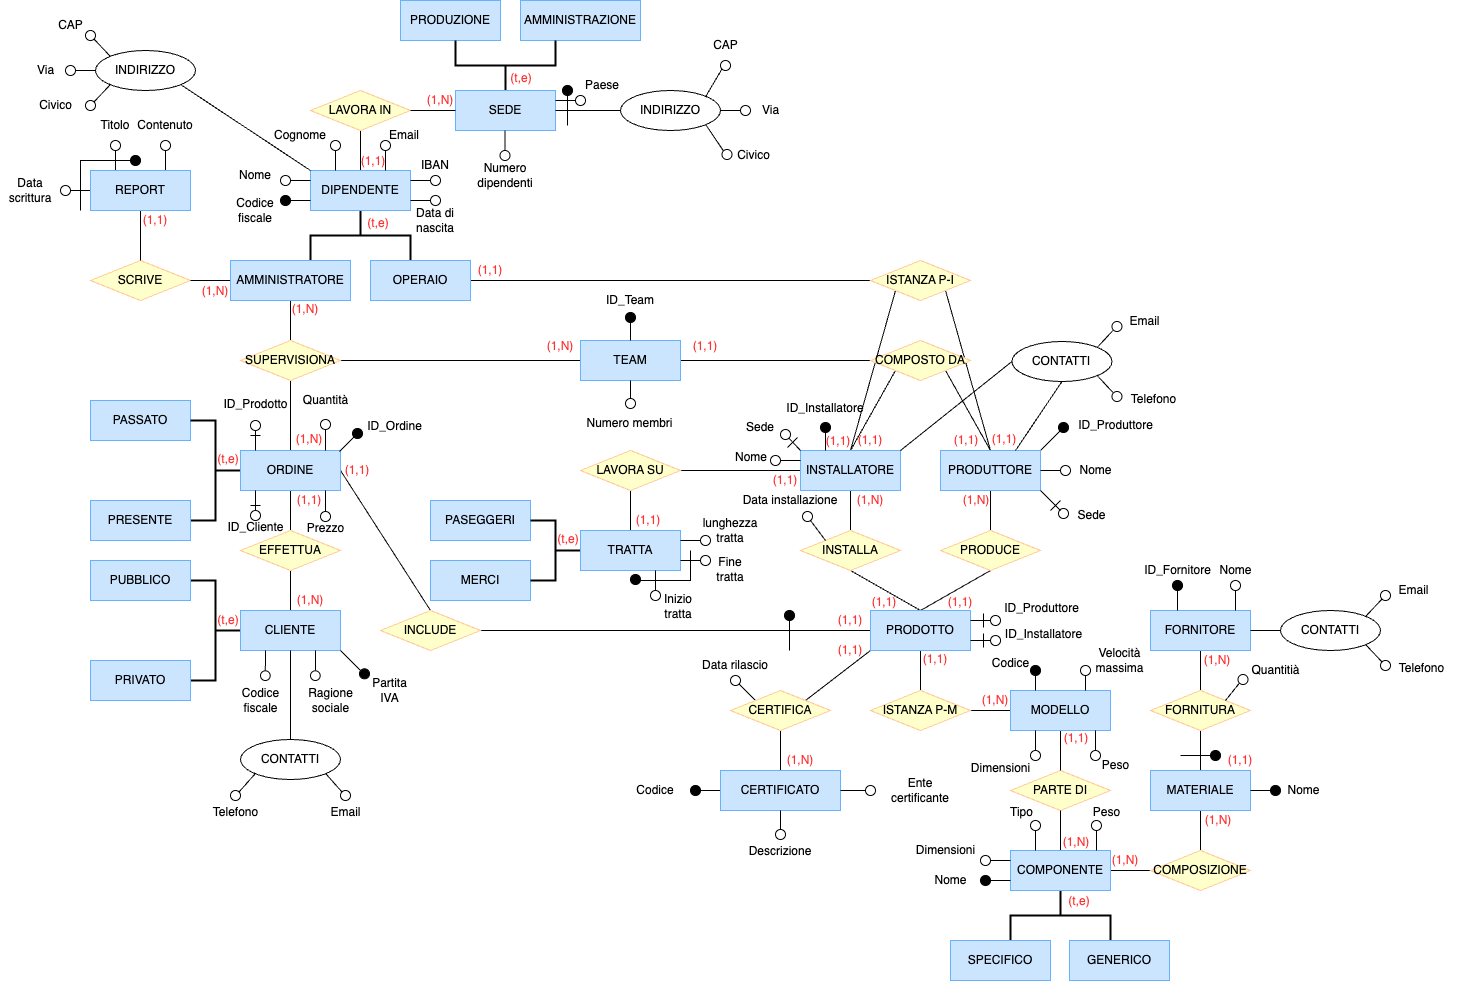
\includegraphics[width=17cm]{images/rivisto_amministratore.drawio.png}\\
    \caption{Schema E-R della vista del Amministratore}
\end{figure}

\newpage

\subsection{Dizionario dei dati}
\subsubsection{Dizionario dei dati per le entità}

\begin{table}[H]
\begin{tabular}{|l|l|l|l|}
\hline
\textbf{Entità}         & \textbf{Descrizione}                                                                             & \textbf{Attributi}                                                                                                   & \textbf{Identificatore}                                              \\ \hline
Cliente                 & \begin{tabular}[c]{@{}l@{}}Ente o azienda richiedente \\ un prodotto\end{tabular}                & \begin{tabular}[c]{@{}l@{}}Codice fiscale, Ragione sociale, \\ Partita IVA, Contatti\end{tabular}                    & Codice univoco                                                       \\ \hline
Privato                 & Ente o azienda privata                                                                           & \begin{tabular}[c]{@{}l@{}}Codice fiscale, Ragione sociale, \\ Partita IVA, Contatti\end{tabular}                    & Partita IVA                                                          \\ \hline
Pubblico                & Ente o azienda pubblica                                                                          & \begin{tabular}[c]{@{}l@{}}Codice fiscale, Ragione sociale, \\ Partita IVA, Contatti\end{tabular}                    & Indice PA                                                            \\ \hline
Ordine                  & Ordine effettuato dal cliente                                                                    & \begin{tabular}[c]{@{}l@{}}ID\_Ordine, ID\_Prodotto, Quantità, \\ Prezzo, ID\_Cliente\end{tabular}                   & ID\_Ordine                                                           \\ \hline
Ordine Presente         & \begin{tabular}[c]{@{}l@{}}Ordine presente effettuato dal \\ cliente\end{tabular}                &                                                                                                                      &                                                                      \\ \hline
Ordine Passato          & \begin{tabular}[c]{@{}l@{}}Ordine passato effettuato dal \\ cliente\end{tabular}                 &                                                                                                                      &                                                                      \\ \hline
Dipendente              & Impiegato dell'azienda                                                                           & \begin{tabular}[c]{@{}l@{}}Codice fiscale, Nome, Cognome, \\ Email, IBAN, Data di nascita, \\ Indirizzo\end{tabular} & Codice fiscale                                                       \\ \hline
Amministratore          & Impiegato di grado più elevato                                                                   &                                                                                                                      &                                                                      \\ \hline
Operaio                 & Lavoratore subordinato                                                                           &                                                                                                                      &                                                                      \\ \hline
Report                  & Documento di informazione                                                                        & Data scrittura, Titolo, Contenuto                                                                                    & \begin{tabular}[c]{@{}l@{}}Titolo, Data\\ scrittura\end{tabular}     \\ \hline
Sede                    & Struttura dell'azienda                                                                           & \begin{tabular}[c]{@{}l@{}}Numero dipendenti, Paese, \\ Indirizzo\end{tabular}                                       & Paese, Indirizzo                                                     \\ \hline
Sede di Produzione      & Reparto di produzione                                                                            &                                                                                                                      &                                                                      \\ \hline
Sede di Amministrazione & Reparto amministrativo                                                                           &                                                                                                                      &                                                                      \\ \hline
Team                    & Squadra di lavoro                                                                                & ID\_Team, Numero membri                                                                                              & ID\_Team                                                             \\ \hline
Installatore            & \begin{tabular}[c]{@{}l@{}}Addetto all'installazione del\\ prodotto\end{tabular}                 & \begin{tabular}[c]{@{}l@{}}ID\_Installatore, Sede, Nome, \\ Contatti\end{tabular}                                    & ID\_Installatore                                                     \\ \hline
Produttore              & \begin{tabular}[c]{@{}l@{}}Addetto alla realizzazione del \\ prodotto\end{tabular}               & \begin{tabular}[c]{@{}l@{}}ID\_Produttore, Sede, Nome, \\ Contatti\end{tabular}                                      & ID\_Produttore                                                       \\ \hline
Tratta                  & Percorso del treno                                                                               & \begin{tabular}[c]{@{}l@{}}Lunghezza tratta, Inizio tratta, \\ Fine tratta\end{tabular}                              & \begin{tabular}[c]{@{}l@{}}Inizio tratta,\\ Fine tratta\end{tabular} \\ \hline
Tratta Passeggeri       & \begin{tabular}[c]{@{}l@{}}Percorso per treni addetti al \\ trasporto di passeggeri\end{tabular} &                                                                                                                      &                                                                      \\ \hline
Tratta Merci            & \begin{tabular}[c]{@{}l@{}}Percorso per treni addetti al \\ trasporti di merci\end{tabular}      &                                                                                                                      &                                                                      \\ \hline
Prodotto                & Oggetto prodotto dall'azienda                                                                    & ID\_Produttore, ID\_Installatore                                                                                     & Ordine                                                               \\ \hline
Modello                 & Variante specifica del prodotto                                                                  & \begin{tabular}[c]{@{}l@{}}Codice, Velocità massima, Peso, \\ Dimensioni\end{tabular}                                & Codice                                                               \\ \hline
Certificato             & \begin{tabular}[c]{@{}l@{}}Documento che attesta la\\ conformità ambientale\end{tabular}         & \begin{tabular}[c]{@{}l@{}}Codice, Descrizione, Ente \\ certificante\end{tabular}                                    & Codice                                                               \\ \hline
Componente              & Parte del prodotto                                                                               & Nome, Dimensioni, Tipo, Peso                                                                                         & Nome                                                                 \\ \hline
Componente Specifico    & \begin{tabular}[c]{@{}l@{}}Componente specifico di un\\ determinato modello\end{tabular}         &                                                                                                                      &                                                                      \\ \hline
Componente Generico     & \begin{tabular}[c]{@{}l@{}}Componente presente in ogni \\ modello\end{tabular}                   &                                                                                                                      &                                                                      \\ \hline
Materiale               & Materia prima per componenti                                                                     & Nome                                                                                                                 & Fornitore                                                            \\ \hline
Fornitore               & Terzo che fornisce i materiali                                                                   & ID\_Fornitore, Nome, Contatti                                                                                        & ID\_Fornitore                                                        \\ \hline
\end{tabular}
\end{table}

\subsubsection{Dizionario dei dati per le relazioni}

\begin{table}[H]
\begin{tabular}{|l|l|l|l|}
\hline
\textbf{Relazioni} & \textbf{Descrizione}                                                                                    & \textbf{Entità Coinvolte}                                                                   & \textbf{Attributi} \\ \hline
Effettua           & Effettuare un ordine                                                                                    & \begin{tabular}[c]{@{}l@{}}Cliente (1,N)\\ Ordine (1,1)\end{tabular}                        & -                  \\ \hline
Supervisiona       & Supervisione Team o Ordine                                                                              & \begin{tabular}[c]{@{}l@{}}Amministratore (1,N)\\ Team (1,N) / Ordine (1,N)\end{tabular}    & -                  \\ \hline
Include            & Inclusione del prodotto nell'ordine                                                                     & \begin{tabular}[c]{@{}l@{}}Ordine (1,1)\\ Prodotto (1,1)\end{tabular}                       & -                  \\ \hline
Scrive             & Scrittura report                                                                                        & \begin{tabular}[c]{@{}l@{}}Amministratore (1,N)\\ Report (1,1)\end{tabular}                 & -                  \\ \hline
Lavora in          & Relazione tra dipendente e sede                                                                         & \begin{tabular}[c]{@{}l@{}}Dipendente (1,1)\\ Sede (1,N)\end{tabular}                       & -                  \\ \hline
Lavora su          & \begin{tabular}[c]{@{}l@{}}Partecipazione a installazione su \\ una tratta\end{tabular}                 & \begin{tabular}[c]{@{}l@{}}Installatore (1,1)\\ Tratta (1,1)\end{tabular}                   & -                  \\ \hline
Istanza P-I        & Associazione Prodotto - Installatore                                                                    & \begin{tabular}[c]{@{}l@{}}Operaio (1,1)\\ Produttore (1,1) / Installatore (1,1)\end{tabular} & -                  \\ \hline
Composto da        & \begin{tabular}[c]{@{}l@{}}Relazione di composizione dei\\ team di installatori/produttori\end{tabular} & \begin{tabular}[c]{@{}l@{}}Team (1,1)\\ Installatore (1,1) / Produttore (1,1)\end{tabular}  & -                  \\ \hline
Installa           & Installazione del prodotto                                                                              & \begin{tabular}[c]{@{}l@{}}Installatore (1,N)\\ Prodotto (1,1)\end{tabular}                 & Data installazione \\ \hline
Produce            & Produzione del prodotto                                                                                 & \begin{tabular}[c]{@{}l@{}}Produttore (1,N)\\ Prodotto (1,1)\end{tabular}                   & -                  \\ \hline
Certifica          & Certificazione del prodotto                                                                             & \begin{tabular}[c]{@{}l@{}}Prodotto (1,1)\\ Certificato (1,N)\end{tabular}                  & Data rilascio      \\ \hline
Istanza P-M        & Associazione Prodotto - Modello                                                                         & \begin{tabular}[c]{@{}l@{}}Prodotto (1,1)\\ Modello (1,N)\end{tabular}                      & -                  \\ \hline
Parte di           & 'Componente' parte di un modello                                                                          & \begin{tabular}[c]{@{}l@{}}Modello (1,1)\\ 'Componente' (1,N)\end{tabular}                    & -                  \\ \hline
Composizione       & \begin{tabular}[c]{@{}l@{}}Relazione tra componente e \\ materiale\end{tabular}                         & \begin{tabular}[c]{@{}l@{}}'Componente' (1,N)\\ Materiale (1,N)\end{tabular}                  & -                  \\ \hline
Fornitura          & Fornitura dei materiali                                                                                 & \begin{tabular}[c]{@{}l@{}}Materiale (1,1)\\ Fornitore (1,N)\end{tabular}                   & Quantità           \\ \hline
\end{tabular}
\end{table}

\subsubsection{Vincoli non esprimibili}

\begin{table}[H]
\centering
\begin{tabular}{|c|}
\hline
\textbf{Vincoli non esprimibili}                                        \\ \hline
Un ordine passato non può essere modificato.                            \\ \hline
Un prodotto non può avere più di 1000 unità in magazzino.               \\ \hline
Un Amministratore che supervisiona un Team deve far parte di quel Team. \\ \hline
Un prodotto può essere installato solo su tratte compatibili.           \\ \hline
Un certificato può essere rilasciato solo se il prodotto è stato installato\\
e collaudato con esito positivo. \\ \hline
La quantità totale di materiali usati in un ordine non deve superare\\
la disponibilità in magazzino della sede fornitrice. \\ \hline
Non si possono generare certificati se il numero di componenti del\\
prodotto non corrisponde a quello previsto dal modello. \\ \hline
\end{tabular}
\end{table}

\section{Progettazione Logica}

\subsection{Ristrutturazione schema E-R}

\subsubsection{Modifiche}
Rinominazioni e modifiche di attributi e relazioni vari attributti, vedi schema finale.

\subsubsection{Eliminazione delle generalizzazioni}
\begin{enumerate}
    \item L'entità 'Cliente' accorpa le entità 'Privato' e 'Pubblico' attaverso l'attributo 'Tipo' dato che gli accessi e operazioni tra queste entità sono gli stessi.
    \item L'entità 'Ordine' accorpa le entità 'Ordine Presente' e 'Ordine Passato' attaverso l'attributo 'Stato' dato che gli accessi e operazioni tra queste entità sono gli stessi.
    \item L'entità 'Sede' accorpa le entità 'Sede Amministrativa' e 'Sede di Produzione' attaverso l'attributo 'Tipo' dato che gli accessi e operazioni tra queste entità sono gli stessi.
    \item L'entità 'Componente' accorpa le entità 'Componente Specifico' e 'Componente Generico' attaverso l'attributo 'Tipo' dato che gli accessi e operazioni tra queste entità sono gli stessi.
    \item L'entità 'Dipendente' accorpa l'entità 'Operaio' dato che gli accessi e operazioni tra queste entità sono gli stessi. L'entità 'Amministratore' è stata mantenuta separata in quanto ha accessi e operazioni diverse rispetto agli altri dipendenti.
    \item L'entità 'Tratta' accorpa le entità 'Tratta Passeggeri' e 'Tratta Merci' attaverso l'attributo 'Tipo' dato che gli accessi e operazioni tra queste entità sono gli stessi.
\end{enumerate}

\subsubsection{Partizionemaneto/accorpamento di entità e relationship}
\begin{enumerate}
    \item L'entità 'Team' accorpa la relationship 'Composto da' attraverso l'attributo 'Tipo'.
\end{enumerate}

\subsection{Carico applicativo}

\begin{figure}[H]
    \begin{table}[H]
        \centering
        \begin{tabular}{|l|l|l|}
            \hline
            \textbf{Concetto} & \textbf{Tipo} & \textbf{Volume} \\ \hline
            Cliente           & E             & 100              \\ \hline
            Ordine            & E             & 1000             \\ \hline
            Amministratore    & E             & 10              \\ \hline
            Report            & E             & 50               \\ \hline
            Team              & E             & 25              \\ \hline
            Dipendente        & E             & 150             \\ \hline
            Sede              & E             & 5               \\ \hline
            Prodotto          & E             & 5000            \\ \hline
            Installatore      & E             & 100             \\ \hline
            Produttore        & E             & 250             \\ \hline
            Tratta            & E             & 5               \\ \hline
            Modello           & E             & 5               \\ \hline
            Certificato       & E             & 5               \\ \hline
            Componente        & E             & 1000             \\ \hline
            Materiale         & E             & 500              \\ \hline
            Fornitore         & E             & 100              \\ \hline
            Composizione      & R             & 2500           \\ \hline
            Fornitura         & R             & 1000             \\ \hline
            Installazione     & R             & 1800            \\ \hline
            Produzione        & R             & 1500            \\ \hline
        \end{tabular}
        \caption{Tabella dei volumi}
    \end{table}
\end{figure}

Legenda:
\begin{itemize}
    \item E = Entità
    \item R = Relazione
\end{itemize}

\begin{figure}[H]
    \centering
    \begin{tabular}{|l|l|l|l|}
        \hline
        \textbf{\#} & \textbf{Operazione} & \textbf{Tipo} & \textbf{Frequenza} \\
        \hline
        1  & Inserimento nuovo prodotto & I & 1/mese \\
        2  & Visualizza componenti di un prodotto & C & 30/giorno \\
        3  & Inserimento nuova tratta & I & 1/anno \\
        4  & Inserimento nuovo cliente & I & 1/mese \\
        5  & Visualizzazione prodotti di un ordine & C & 20/giorno \\
        6  & Visualizzazione attributi Prodotto & C & 50/giorno \\
        7  & Inserimento di un nuovo componente & I & 5/mese \\
        8  & Inserimento di un ordine & I & 30/mese \\
        9  & Inserimento nuovo certificato di un prodotto & I & 2/mese \\
        10 & Inserimento nuovo dipendente & I & 1/mese \\
        11 & Visualizzazione attributi Modello & C & 10/giorno \\
        12 & Visualizzazione attributi Componente & C & 40/giorno \\
        13 & Inserimento di un nuovo report & I & 2/mese \\
        14 & Visualizzazione attributi cliente & C & 10/giorno \\
        15 & Inserimento nuovo team & I & 3/mese \\
        16 & Aggiornamento attributi ordine & A & 5/mese \\
        17 & Aggiornamento attributi componente & A & 10/mese \\
        18 & Inserimento nuovo materiale & I & 10/mese \\
        19 & Aggiornamento attributi fornitore & A & 3/mese \\
        20 & Inserimento nuova sede & I & 1/anno \\
        21 & Calcolo numero dipendenti in una sede & C & 5/giorno \\
        22 & Aggiornamento prezzo componente & A & 10/mese \\
        23 & Eliminazione di un cliente & E & 1/anno \\
        24 & Visualizzazione prezzo prodotto & C & 100/giorno \\
        25 & Modifica prezzo componente & A & 5/mese \\
        26 & Visualizzazione attributi dipendente & C & 10/giorno \\
        27 & Visualizzazione attributi fornitore & C & 10/giorno \\
        \hline
    \end{tabular}
    \caption{Tabella delle operazioni}
\end{figure}


Legenda:
\begin{itemize}
    \item C = Consultazione
    \item I = Inserimento
    \item A = Aggiornamento
    \item E = Eliminazione
\end{itemize}

\subsection{Valutazione dei costi dei dati derivati}
Approssimiamo un mese = 30 giorni.

\newpage

\subsubsection{Valutazioni dei costi per il dato derivato 'Numero componenti di un prodotto'}

\begin{table}[H]
\centering
\begin{tabular}{|l|l|l|l|}
\hline
        & \textbf{Concetto}                                                & \textbf{Accessi}                              & \textbf{Tipo}                                 \\ \hline
\textbf{\begin{tabular}[c]{@{}l@{}}Operazione 1\\ 6 accessi in scrittura\\ 12 operazioni x 1/mese = 12 operazioni/mese\end{tabular}} & \begin{tabular}[c]{@{}l@{}}PRODOTTO \\ COMPOSIZIONE\end{tabular} & \begin{tabular}[c]{@{}l@{}}1\\ 5\end{tabular} & \begin{tabular}[c]{@{}l@{}}S\\ S\end{tabular} \\ \hline
\textbf{\begin{tabular}[c]{@{}l@{}}Operazione 2\\ 1 accesso in lettura\\ 1 operazione x 30/giorno = 900 operazioni/mese\end{tabular}}    & PRODOTTO                                                         & 1                                             & L                                             \\ \hline
\textbf{\begin{tabular}[c]{@{}l@{}}Operazione 7\\ 2 accessi in scrittura\\ 4 operazioni x 5/mese = 20 operazioni/mese\end{tabular}}   & \begin{tabular}[c]{@{}l@{}}COMPOSIZIONE \\ PRODOTTO\end{tabular} & \begin{tabular}[c]{@{}l@{}}1\\ 1\end{tabular} & \begin{tabular}[c]{@{}l@{}}S\\ S\end{tabular} \\ \hline
\end{tabular}
\caption{Con dato derivato}
\end{table}

Carico mensile $\approx 932\text{ accessi/mese}$.

\begin{table}[H]
    \centering
    \begin{tabular}{|l|l|l|l|}
        \hline
        & \textbf{Concetto}                                                  & \textbf{Accessi}                              & \textbf{Tipo}                                 \\ \hline
        \textbf{\begin{tabular}[c]{@{}l@{}}Operazione 1\\ 6 accessi in scrittura\\ 12 operazioni x 1/mese = 12 operazioni/mese\end{tabular}} & \begin{tabular}[c]{@{}l@{}}PRODOTTO \\ COMPOSIZIONE\end{tabular}   & \begin{tabular}[c]{@{}l@{}}1\\ 5\end{tabular} & \begin{tabular}[c]{@{}l@{}}S\\ S\end{tabular} \\ \hline
        \textbf{\begin{tabular}[c]{@{}l@{}}Operazione 2\\ 5 accesso in lettura\\ 5 operazioni x 30/giorno = 4500 operazioni/mese\end{tabular}}   & \begin{tabular}[c]{@{}l@{}}COMPOSIZIONE \\ COMPONENTE\end{tabular} & \begin{tabular}[c]{@{}l@{}}5\\ 5\end{tabular} & \begin{tabular}[c]{@{}l@{}}L\\ L\end{tabular} \\ \hline
        \textbf{\begin{tabular}[c]{@{}l@{}}Operazione 7\\ 1 accessi in scrittura\\ 2 operazioni x 5/mese = 10 operazioni/mese\end{tabular}}   & COMPOSIZIONE                                                       & 1                                             & S                                             \\ \hline
    \end{tabular}
    \caption{Senza dato derivato}
\end{table}

Carico mensile $\approx 4522\text{ accessi/mese}$.

\textbf{Conviene mantenere il dato derivato.}

\subsubsection{Valutazioni dei costi per il dato derivato 'Prezzo' dai componenti}

\begin{table}[H]
    \centering
    \begin{tabular}{|l|l|l|l|}
        \hline
        & \textbf{Concetto}                                                              & \textbf{Accessi}                                  & \textbf{Tipo}                                     \\ \hline
        \textbf{\begin{tabular}[c]{@{}l@{}}Operazione 1\\ 10 accessi in scrittura\\ 16 operazioni x 1/mese = 16 operazioni/mese\end{tabular}} & \begin{tabular}[c]{@{}l@{}}COMPONENTE \\ COMPOSIZIONE \\ PRODOTTO\end{tabular} & \begin{tabular}[c]{@{}l@{}}5\\ 5\\ 1\end{tabular} & \begin{tabular}[c]{@{}l@{}}L\\ S\\ S\end{tabular} \\ \hline
        \textbf{\begin{tabular}[c]{@{}l@{}}Operazione 24\\ 1 accesso in lettura\\ 1 operazione x 100/giorno = 3000 operazioni/mese\end{tabular}}   & PRODOTTO                                                                       & 5                                                 & L                                                 \\ \hline
        \textbf{\begin{tabular}[c]{@{}l@{}}Operazione 25\\ 2 accessi in scrittura\\ 4 operazioni x 5/mese = 20 operazioni/mese\end{tabular}}   & \begin{tabular}[c]{@{}l@{}}COMPONENTE \\ PRODOTTO\end{tabular}                 & \begin{tabular}[c]{@{}l@{}}1\\ 1\end{tabular}     & \begin{tabular}[c]{@{}l@{}}S\\ S\end{tabular}     \\ \hline
    \end{tabular}
    \caption{Con dato derivato}
\end{table}

Carico mensile $\approx 3036\text{ accessi/mese}$.

\begin{table}[H]
    \centering
    \begin{tabular}{|l|l|l|l|}
        \hline
        & \textbf{Concetto}                                                  & \textbf{Accessi}                              & \textbf{Tipo}                                 \\ \hline
        \textbf{\begin{tabular}[c]{@{}l@{}}Operazione 1\\ 6 accessi in scrittura\\ 12 operazioni x 1/mese = 12 operazioni/mese\end{tabular}}         & \begin{tabular}[c]{@{}l@{}}COMPOSIZIONE \\ PRODOTTO\end{tabular}   & \begin{tabular}[c]{@{}l@{}}5\\ 1\end{tabular} & \begin{tabular}[c]{@{}l@{}}S\\ S\end{tabular} \\ \hline
        \textbf{\begin{tabular}[c]{@{}l@{}}Operazione 24\\ 10 accesso in lettura\\ 10 operazione x 100/giorno = 30000 operazioni/mese\end{tabular}} & \begin{tabular}[c]{@{}l@{}}COMPOSIZIONE \\ COMPONENTE\end{tabular} & \begin{tabular}[c]{@{}l@{}}5\\ 5\end{tabular} & \begin{tabular}[c]{@{}l@{}}L\\ L\end{tabular} \\ \hline
        \textbf{\begin{tabular}[c]{@{}l@{}}Operazione 25\\ 2 accessi in scrittura\\ 4 operazioni x 5/mese = 20 operazioni/mese\end{tabular}}         & COMPOSIZIONE                                                       & 1                                             & S                                             \\ \hline
    \end{tabular}
    \caption{Senza dato derivato}
\end{table}

Carico mensile $\approx 30032\text{ accessi/mese}$.

\textbf{NON conviene mantenere il dato derivato.}

\subsection{Traduzione dello schema E-R ristrutturato in modello relazionale}

\begin{figure}[H]
    \centering
    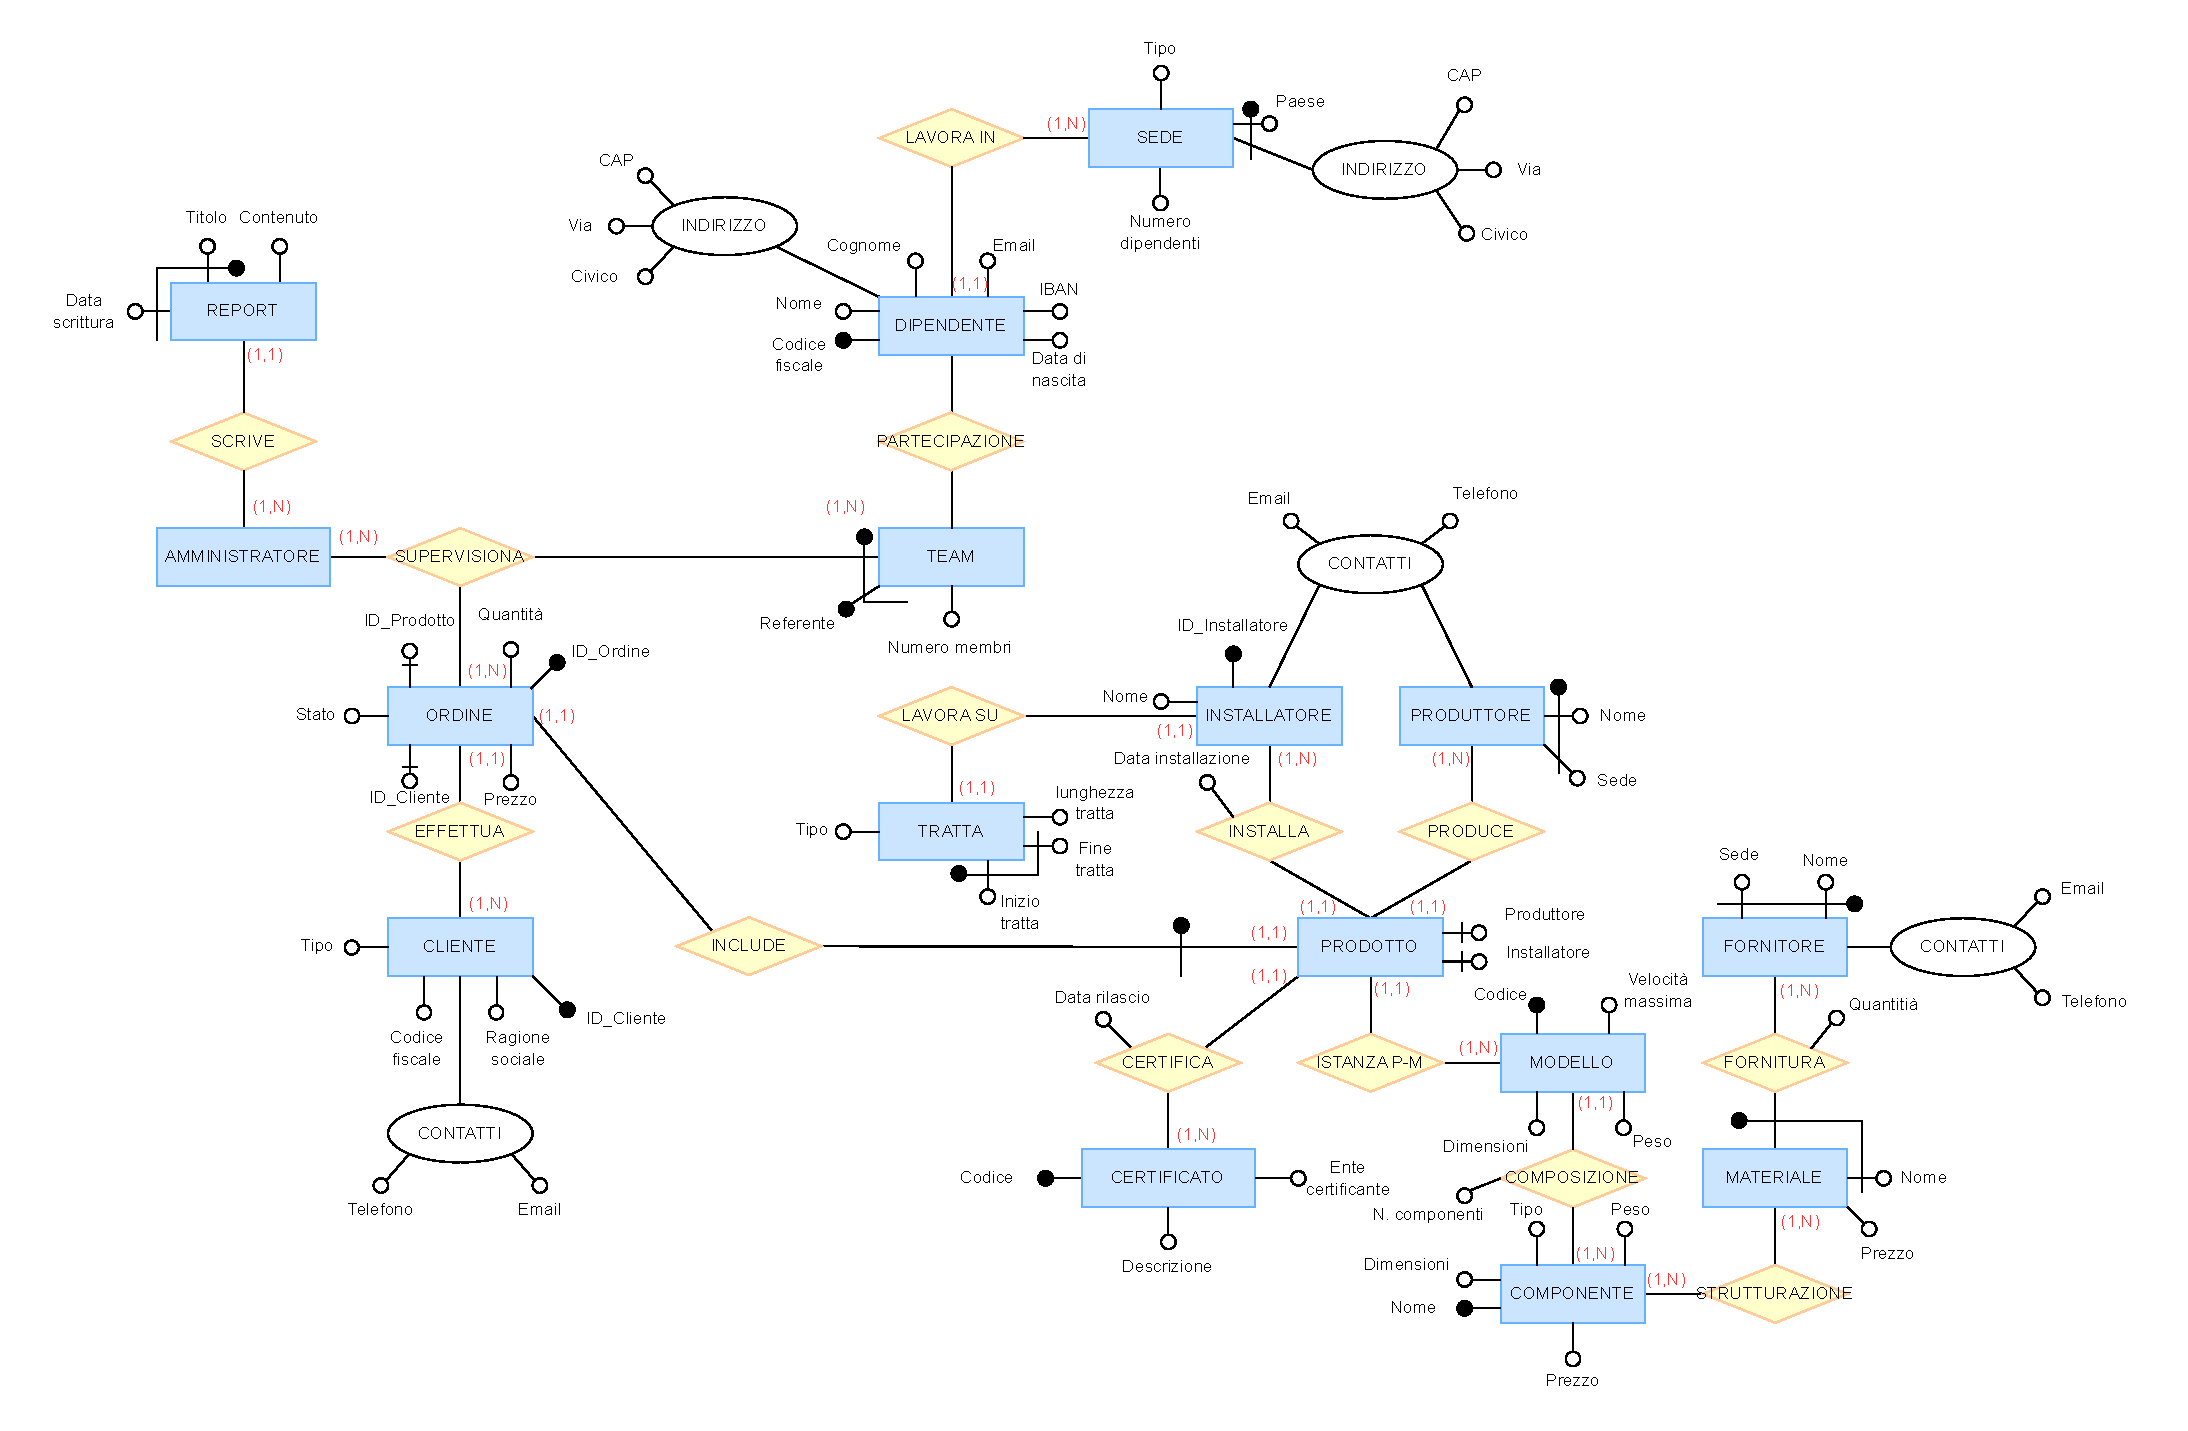
\includegraphics[width=24.25cm, angle=-90]{images/ristrutturato.drawio.pdf}
    \caption{Schema E-R della vista del Amministratore}
\end{figure}

\newpage

\textbf{Cliente}(\underline{\text{ID\_Cliente}}, \text{Ragione sociale}, \text{Codice fiscale}, \text{Telefono}, \text{Email}, \text{Tipo})\\


\textbf{Ordine}(\underline{\text{ID\_Ordine}}, \text{Prezzo},\, \text{Quantità},\, \text{Stato},\, \text{Email},\, \text{Tipo}, \text{Prodotto})\\
\indent\indent \textbf{FK}: ID\_Prodotto \textbf{REFERENCES} Prodotto\\
\indent\indent \textbf{FK}: ID\_Cliente \textbf{REFERENCES} Cliente\\


\textbf{Amministratore}(\underline{\text{ID\_Cliente}}, \text{Ragione sociale}, \text{Codice fiscale}, \text{Telefono}, \text{Email}, \text{Tipo})\\


\textbf{Report}(\underline{\text{Data scrittura, Titolo}}, \text{Contenuto})\\


\textbf{Sede}(\underline{\text{Paese, CAP, Via, Civico}}, \text{Tipo}, \text{Numero dipendenti})\\


\textbf{Dipendente}(\underline{\text{Codice fiscale}}, \text{Nome}, \text{Cognome}, \text{IBAN}, \text{Data di nascita}, \text{Email}, \text{Via}, \text{CAP}, \text{Civico})\\


\textbf{Team}(\underline{\text{Referente, Amministratore, Sede}}, \text{Numero membri})\\
\indent\indent \textbf{FK}: Amministratore \textbf{REFERENCES} Amministratore\\
\indent\indent \textbf{FK}: Sede \textbf{REFERENCES} Sede\\


\textbf{Tratta}(\underline{\text{Inizio tratta, Fine tratta}}, \text{Lunghezza tratta}, \text{Tipo})\\


\textbf{Installatore}(\underline{\text{ID\_Installatore}}, \text{Nome}, \text{Email}, \text{Telefono})\\


\textbf{Produttore}(\underline{\text{Nome, Sede}}, \text{Telefono}, \text{Email})\\
\indent\indent \textbf{FK}: Sede \textbf{REFERENCES} Sede\\


\textbf{Prodotto}(\underline{\text{Ordine}}, \text{Installatore}, \text{Produttore})\\
\indent\indent \textbf{FK}: Ordine \textbf{REFERENCES} Ordine\\
\indent\indent \textbf{FK}: Installatore \textbf{REFERENCES} Installatore\\
\indent\indent \textbf{FK}: Produttore \textbf{REFERENCES} Produttore\\


\textbf{Certificato}(\underline{\text{Codice}}, \text{Descrizione}, \text{Ente certificante})\\


\textbf{Modello}(\underline{\text{Codice}}, \text{Velocità massima}, \text{Peso}, \text{Dimensioni})\\


\textbf{Componente}(\underline{\text{Nome}}, \text{Peso}, \text{Tipo}, \text{Dimensioni}, \text{Prezzo})\\


\textbf{Materiale}(\underline{\text{Nome, Fornitore}}, \text{Prezzo})\\
\indent\indent \textbf{FK}: Fornitore \textbf{REFERENCES} Fornitore\\


\textbf{Fornitore}(\underline{\text{Nome, Sede}}, \text{Email}, \text{Telefono})\\
\indent\indent \textbf{FK}: Sede \textbf{REFERENCES} Sede\\

\textbf{Installa}(\underline{\text{Installatore, Prodotto}}, \text{Data installazione})\\
\indent\indent \textbf{FK}: Installatore \textbf{REFERENCES} Installatore\\
\indent\indent \textbf{FK}: Prodotto \textbf{REFERENCES} Prodotto\\

\textbf{Certifica}(\underline{\text{Certificato, Prodotto}}, \text{Data rilascio})\\
\indent\indent \textbf{FK}: Certificato \textbf{REFERENCES} Certificato\\
\indent\indent \textbf{FK}: Prodotto \textbf{REFERENCES} Prodotto\\

\textbf{Fornitura}(\underline{\text{Fornitore, Materiale}}, \text{Quantità})\\
\indent\indent \textbf{FK}: Fornitore \textbf{REFERENCES} Fornitore\\
\indent\indent \textbf{FK}: Materiale \textbf{REFERENCES} Materiale\\

\textbf{Composizione}(\underline{\text{Modello, Componente}}, \text{Numero componenti})\\
\indent\indent \textbf{FK}: Fornitore \textbf{REFERENCES} Fornitore\\
\indent\indent \textbf{FK}: Materiale \textbf{REFERENCES} Materiale\\
% \section{Methodology}
% This section has a subsection.
% \subsection{Subsection}
% This subsection contains \autoref{eq:1}.
% \begin{equation}
% \label{eq:1}
%     h(r) = \cfrac{Q}{2\pi T} \ln(\cfrac{r_i}{r_0})+h_0
% \end{equation}

% \section{Results}

% l

% \section{Discussion}

% As shown in previous studies, the proposed system has significant potential.

\newpage
\addcontentsline{toc}{section}{References}
\bibliographystyle{apalike}
\bibliography{ref}

% \newpage
% \appendix
% \section{Additional graphs and data}

\end{document}


%All other official TU Delft colours
\definecolor{donkerblauw}{RGB}{12, 35, 64}
\definecolor{turkoois}{RGB}{0, 184, 200}
\definecolor{blauw}{RGB}{0, 118, 194}
\definecolor{paars}{RGB}{111, 29, 119}
\definecolor{roze}{RGB}{239, 96, 163}
\definecolor{framboos}{RGB}{165, 0, 52}
\definecolor{rood}{RGB}{224, 60, 49}
\definecolor{oranje}{RGB}{237, 104, 66}
\definecolor{geel}{RGB}{255, 184, 28}
\definecolor{lichtgroen}{RGB}{108, 194, 74}
\definecolor{donkergroen}{RGB}{0, 155, 119}
%You can use these to change the hyperlink colour or the colour of the header or whatever. Glück Auf!
\end{itemize}hapter{Definizione e Analisi dei Requisiti}
